\chapter{Trajectory Optimization in Practice}
\label{ch:traj-opt}

\epigraph{Theory without practice is empty. Practice without theory is blind.}{}

\section{DDP/iLQR Implementation}

Differential Dynamic Programming (DDP) and iterative Linear Quadratic Regulator (iLQR) are
related algorithms for trajectory optimization \cite{Mayne1966, jacobson1970dpp}. They solve
the finite-horizon optimal control problem by iteratively linearizing around a nominal
trajectory and solving quadratic subproblems. Figure~\ref{fig:ilqr-loop} shows the algorithm structure.

iLQR is a numerical method for implementing the feedback synthesis results from Agrachev \&
Sachkov \cite{AgrachevSachkov2004}, Chapter~6: it iteratively computes the optimal feedback law
via local linearization and quadratic approximation of the cost. The backward-pass computation
of gains $K(t)$ corresponds to the solution of the Riccati equation, a central object in their
optimal control theory.

\begin{figure}[h]
  \centering
  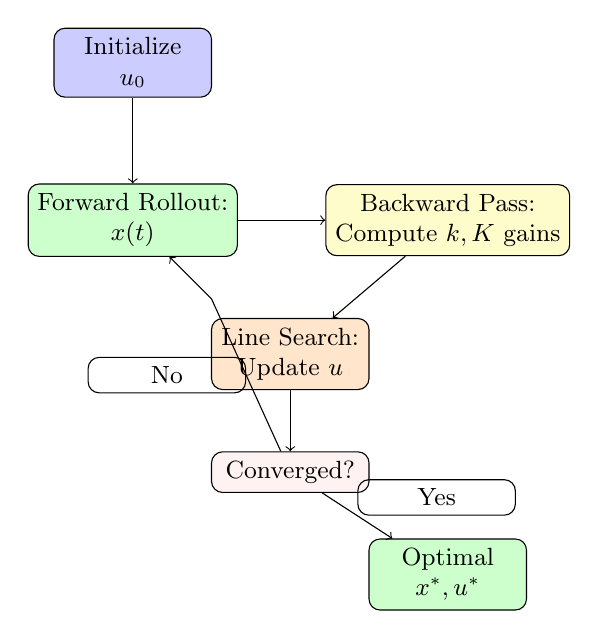
\begin{tikzpicture}[
    every node/.style={align=center, draw, rounded corners, minimum width=2cm, text centered, font=\small},
    ]
    % Initial trajectory
    \node[fill=blue!20] (init) at (0, 4) {Initialize\\$\bm{u}_0$};

    % Forward pass
    \node[fill=green!20] (forward) at (0, 2) {Forward Rollout:\\$\bm{x}(t)$};

    % Backward pass
    \node[fill=yellow!20] (backward) at (4, 2) {Backward Pass:\\Compute $k, K$ gains};

    % Line search
    \node[fill=orange!20] (linesearch) at (2, 0.3) {Line Search:\\Update $\bm{u}$};

    % Convergence check
    \node[fill=pink!20] (converge) at (2, -1.2) {Converged?};

    % Exit
    \node[fill=green!20] (exit) at (4, -2.5) {Optimal\\$\bm{x}^*, \bm{u}^*$};

    % Arrows
    \draw[->] (init) -- (forward);
    \draw[->] (forward) -- (backward);
    \draw[->] (backward) -- (linesearch);
    \draw[->] (linesearch) -- (converge);
    \draw[->] (converge) -- node[align=center, left] {No} (1, 1) -- (forward);
    \draw[->] (converge) -- node[align=center, above right] {Yes} (exit);
  \end{tikzpicture}
  \caption{iLQR algorithm loop: initialize control trajectory, forward rollout
    to compute state trajectory, backward pass to compute feedback gains,
    line search to update controls, and convergence check.}
  \label{fig:ilqr-loop}
\end{figure}

Here we implement iLQR end-to-end:
Differential Dynamic Programming (Volume~I, Chapter~5) is the workhorse for
trajectory optimization. Here we implement it end-to-end:

\begin{lstlisting}[language=Python, caption={iLQR implementation for trajectory optimization.}]
import numpy as np
from typing import Callable, Tuple

def ilqr_solve(
    dynamics: Callable,
    cost_running: Callable,
    cost_terminal: Callable,
    x0: np.ndarray,
    u_init: np.ndarray,
    n_iterations: int = 50,
    regularization: float = 1e-6
) -> Tuple[np.ndarray, np.ndarray, list[float]]:
    """Iterative Linear Quadratic Regulator.

    Parameters
    ----------
    dynamics : callable
        (x, u) -> x_next, (A, B) Jacobians
    cost_running : callable
        (x, u) -> (cost, lx, lu, lxx, luu, lux)
    cost_terminal : callable
        x -> (cost, lx, lxx)
    x0 : np.ndarray
        Initial state.
    u_init : np.ndarray, shape (T, m)
        Initial control trajectory.
    n_iterations : int
        Maximum iterations.
    regularization : float
        Regularization for Quu inversion.

    Returns
    -------
    Tuple
        (x_traj, u_traj, costs)
    """
    T, m = u_init.shape
    n = len(x0)

    # Forward rollout with initial controls
    x_traj = np.zeros((T + 1, n))
    x_traj[0] = x0
    u_traj = u_init.copy()

    for t in range(T):
        x_next, _ = dynamics(x_traj[t], u_traj[t])
        x_traj[t + 1] = x_next

    costs = []

    for iteration in range(n_iterations):
        # Compute total cost
        total_cost = sum(
            cost_running(x_traj[t], u_traj[t])[0]
            for t in range(T)
        ) + cost_terminal(x_traj[T])[0]
        costs.append(total_cost)

        # Backward pass
        Vx_next, Vxx_next = cost_terminal(x_traj[T])[1:]
        k_gains = np.zeros((T, m))
        K_gains = np.zeros((T, m, n))

        for t in range(T - 1, -1, -1):
            _, (A, B) = dynamics(x_traj[t], u_traj[t])
            _, lx, lu, lxx, luu, lux = cost_running(
                x_traj[t], u_traj[t]
            )

            Qx = lx + A.T @ Vx_next
            Qu = lu + B.T @ Vx_next
            Qxx = lxx + A.T @ Vxx_next @ A
            Quu = luu + B.T @ Vxx_next @ B + regularization * np.eye(m)
            Qux = lux + B.T @ Vxx_next @ A

            Quu_inv = np.linalg.inv(Quu)
            k_gains[t] = -Quu_inv @ Qu
            K_gains[t] = -Quu_inv @ Qux

            Vx_next = Qx + K_gains[t].T @ Quu @ k_gains[t]
            Vxx_next = Qxx + K_gains[t].T @ Quu @ K_gains[t]

        # Forward pass with line search
        alpha = 1.0
        x_new = np.zeros_like(x_traj)
        u_new = np.zeros_like(u_traj)
        x_new[0] = x0

        for t in range(T):
            dx = x_new[t] - x_traj[t]
            u_new[t] = u_traj[t] + alpha * k_gains[t] + K_gains[t] @ dx
            x_new[t + 1], _ = dynamics(x_new[t], u_new[t])

        x_traj = x_new
        u_traj = u_new

        if iteration > 0 and abs(costs[-1] - costs[-2]) < 1e-6:
            break

    return x_traj, u_traj, costs
\end{lstlisting}

\section{Application: Optimal Pendulum Swing-Up}

The pendulum swing-up is a classic trajectory optimization benchmark. The goal is to
find the minimum-energy torque sequence that brings the pendulum from the downward
(stable) equilibrium to the upright (unstable) equilibrium.

This is a canonical example in Agrachev \& Sachkov \cite{AgrachevSachkov2004} (Chapter~5, Example 5.1):
the pendulum system is an affine control system $\ddot{\theta} = -g\sin\theta + u$, and the swing-up
problem is optimal synthesis: find the control law that minimizes energy while ensuring convergence
to the upright equilibrium. Their theory predicts that the optimal trajectory will exhibit
``bang-bang'' control (maximum torque in one direction) followed by a final feedback phase---
which is exactly what occurs in practice.
The classic control benchmark: swing a pendulum from the hanging position to
the inverted equilibrium.

\section{Application: Golf Swing Optimization}

Applying DDP to a 3-DOF golf model to optimize clubhead speed at impact.

\section*{Exercises}
\begin{enumerate}
  \item Use the iLQR code to solve the pendulum swing-up problem.
  \item Extend to a double pendulum and optimize for maximum tip speed.
  \item Add muscle force constraints and solve the muscle-driven swing-up.
\end{enumerate}
